\documentclass[conference]{IEEEtran}
\IEEEoverridecommandlockouts
% The preceding line is only needed to identify funding in the first footnote. If that is unneeded, please comment it out.
%Template version as of 6/27/2024

\usepackage{cite}
\usepackage{amsmath,amssymb,amsfonts}
\usepackage{algorithmic}
\usepackage{graphicx}
\usepackage{tabularx}
\graphicspath{{figuras/}}
\usepackage{textcomp}
\usepackage{xcolor}
\usepackage[hidelinks]{hyperref}
\def\BibTeX{{\rm B\kern-.05em{\sc i\kern-.025em b}\kern-.08em
    T\kern-.1667em\lower.7ex\hbox{E}\kern-.125emX}}
\begin{document}

\title{Avaliação de Desempenho e Dimensionamento de Máquinas Virtuais em Nuvem com Redes de Petri Estocásticas}

\author{
\IEEEauthorblockN{Rais Eliete de Sousa}
\IEEEauthorblockA{
\textit{Universidade Federal do Piauí}\\
Picos-PI, Brasil\\
rais.sousa@ufpi.edu.br}
}

\maketitle

\renewcommand{\abstractname}{Resumo}
\begin{abstract}
Este trabalho avalia o dimensionamento de máquinas virtuais
em nuvem por meio de um modelo de Redes de Petri Estocásticas
implementado no Jupiter Analytics. Simulações estacionárias
investigam variações na demanda, na quantidade de VMs e na
capacidade de uma fila compartilhada, considerando vazão,
resposta, espera, utilização e descarte. Com vinte tarefas
por segundo, ampliar a capacidade de duas para três VMs
reduziu o tempo médio de resposta de 0,5896 s para 0,1445 s.
A ampliação da fila reduziu o descarte, com pequeno aumento
da resposta. Os resultados identificam o processamento como
gargalo sob demanda elevada e indicam três VMs como alternativa
de equilíbrio entre recursos e desempenho no cenário de referência.
\end{abstract}

\renewcommand{\abstractname}{Abstract}
\begin{abstract}
This work evaluates cloud virtual machine capacity planning
through a Stochastic Petri Net model implemented in Jupiter
Analytics. Steady-state simulations investigate changes in
demand, VM count, and shared queue capacity, considering
throughput, response time, waiting time, utilization, and
task rejection. At twenty tasks per second, increasing
capacity from two to three VMs reduced mean response time
from 0.5896 s to 0.1445 s. Increasing queue capacity reduced
rejection, with a small increase in response time. The results
identify processing capacity as the bottleneck under high
demand and indicate three VMs as a trade-off between resources
and performance in the reference scenario.
\end{abstract}

\begin{IEEEkeywords}
Cloud computing, virtual machines, Stochastic Petri Nets,
performance evaluation, capacity planning.
\end{IEEEkeywords}

\section{Introdução}
\label{sec:introducao}

A computação em nuvem permite disponibilizar recursos computacionais para a execução de aplicações e o processamento de tarefas. Nesse ambiente, a quantidade de recursos disponíveis influencia a capacidade de atendimento e a qualidade do serviço oferecido aos usuários. A avaliação de desempenho permite investigar essa relação e apoiar decisões de dimensionamento, considerando a carga de trabalho e os requisitos das aplicações~\cite{ghandour2023computing}. Estudos com serviços executados em máquinas virtuais também evidenciam a importância da caracterização da carga e da análise do tempo de resposta das transações~\cite{juiz2023case}.

Quando todas as máquinas virtuais estão ocupadas, as tarefas recebidas pelo sistema precisam aguardar pelo processamento. O crescimento da demanda pode aumentar essa espera e, consequentemente, o tempo médio de resposta. Em sistemas com fila limitada, também pode ocorrer descarte de tarefas por insuficiência de espaço. Dessa forma, a análise conjunta do tempo de resposta, da utilização dos recursos e da probabilidade de descarte contribui para identificar limitações de capacidade. Ghandour et al.~\cite{ghandour2023computing} avaliam essas medidas para investigar a escalabilidade de recursos em um centro de dados em nuvem. Srivastava e Kumar~\cite{srivastava2023queueing} utilizam modelos de filas para estudar o dimensionamento de recursos em ambientes com contêineres, considerando medidas como tempo de resposta, vazão e descarte.

As Redes de Petri Estocásticas (\textit{Stochastic Petri Nets} --- SPNs) permitem representar a concorrência, a disponibilidade de recursos e a duração das atividades de um sistema. Esse formalismo pode ser empregado para investigar como alterações na demanda e na capacidade afetam o desempenho. Macedo et al.~\cite{macedo2022vanets} utilizam SPNs para avaliar uma arquitetura de comunicação veicular, comparando configurações de recursos sob diferentes taxas de chegada. Essa abordagem de avaliação orienta a construção dos experimentos do presente trabalho.

O objetivo deste trabalho é analisar como a quantidade de máquinas virtuais afeta o tempo médio de resposta das tarefas sob diferentes taxas de chegada. Para isso, é desenvolvido um modelo SPN de um ambiente de computação em nuvem composto por máquinas virtuais idênticas e uma fila compartilhada de capacidade limitada. Cada VM processa uma tarefa por vez, e as tarefas recebidas quando a fila está cheia são descartadas. O modelo é implementado na ferramenta Jupiter Analytics e avaliado por simulação em regime estacionário.

São realizados quatro conjuntos de experimentos, considerando a variação da taxa de chegada, da quantidade de VMs, da capacidade da fila e de combinações de demanda e recursos. Uma análise complementar compara cinco configurações de VMs sob os mesmos níveis de demanda. A avaliação considera a vazão, o tempo médio de resposta, o tempo médio de espera, a utilização das VMs e a probabilidade de descarte. Os resultados são utilizados para identificar limitações de processamento e fundamentar recomendações de dimensionamento para os cenários estudados.

O restante deste artigo está organizado da seguinte forma. A Seção~\ref{sec:arquitetura} apresenta a arquitetura do sistema. A Seção~\ref{sec:modelagem} descreve o modelo SPN, seus parâmetros e as métricas utilizadas. A Seção~\ref{sec:resultados} apresenta o planejamento experimental e discute os resultados. Por fim, a Seção~\ref{sec:conclusao} apresenta as conclusões e as possibilidades de continuidade do estudo.


\section{Arquitetura}
\label{sec:arquitetura}

A Figura~\ref{fig:arquitetura} apresenta a arquitetura do
sistema de processamento de tarefas em nuvem considerado neste
trabalho. O sistema compreende três partes: dispositivos
clientes, admissão e espera, e processamento em nuvem. As
requisições enviadas pelos dispositivos passam pelo controle
de admissão e são encaminhadas para uma fila compartilhada.
As máquinas virtuais disponíveis retiram tarefas dessa fila
para processamento. Após o atendimento, as tarefas deixam
o sistema.

\begin{figure}[!t]
    \centering
    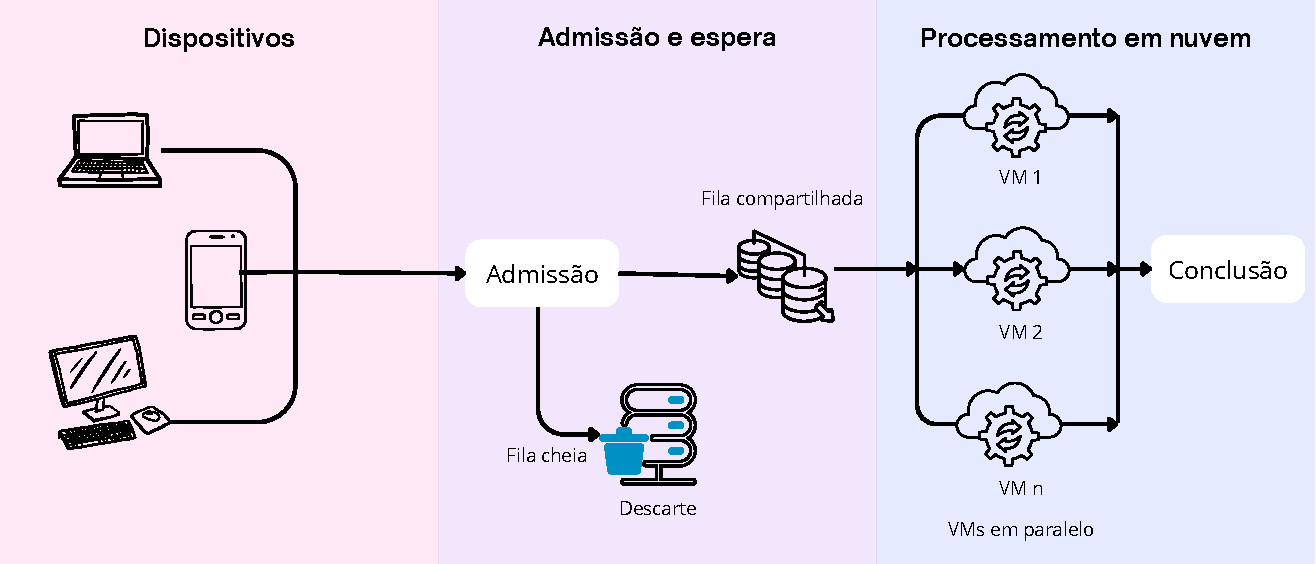
\includegraphics[width=\columnwidth]{arquitetura.pdf}
    \caption{Arquitetura do sistema de processamento de
    tarefas em nuvem.}
    \label{fig:arquitetura}
\end{figure}

\subsection{Dispositivos clientes}

Os dispositivos representam computadores e smartphones
utilizados para acessar uma aplicação em nuvem. Cada
requisição enviada à aplicação é representada como uma tarefa
a ser processada. O modelo considera a demanda agregada desses
dispositivos por meio de uma taxa média de chegada. Dessa
forma, a quantidade de aparelhos ilustrados na figura
representa possíveis origens das requisições, enquanto a
intensidade da demanda é definida como um parâmetro dos
experimentos.

\subsection{Admissão e espera}

O controle de admissão verifica se existe uma posição
disponível na fila. Quando há espaço, a tarefa é admitida e
aguarda uma VM disponível. Caso a fila esteja cheia, a
requisição é descartada, conforme o fluxo indicado na
Figura~\ref{fig:arquitetura}.

A fila é compartilhada pelas VMs e possui capacidade limitada.
Sua capacidade corresponde ao número máximo de tarefas em
espera. Quando uma tarefa inicia o processamento, a posição
que ocupava na fila é liberada para uma nova requisição.
Se houver uma VM disponível no momento da admissão, o
processamento pode começar imediatamente.

\subsection{Processamento em nuvem}

O processamento é realizado por um conjunto de VMs idênticas,
representadas na figura por VM~1, VM~2 e VM~$n$. Cada VM
processa uma tarefa por vez e permanece ocupada até a
conclusão do atendimento. Ao terminar, a tarefa deixa o
sistema e a VM fica disponível para atender outra requisição.

A quantidade de VMs determina o número máximo de tarefas
processadas simultaneamente. A capacidade total do sistema
compreende as posições de espera e os recursos de
processamento. Assim, uma configuração com $B$ vagas na fila
e $n$ VMs pode acomodar até $B+n$ tarefas, considerando as
tarefas em espera e em processamento.

\subsection{Hipóteses e delimitação do sistema}

O modelo considera VMs com a mesma capacidade de processamento
e tarefas pertencentes a uma única classe de serviço. O
atendimento de uma tarefa ocorre integralmente em uma VM.
Os efeitos de comunicação, armazenamento e interferência
entre VMs que compartilham um equipamento físico ficam fora
do escopo da avaliação.

No cenário de referência, são consideradas três VMs, vinte
vagas na fila, taxa média de chegada de vinte tarefas por
segundo e tempo médio de serviço de 0,1~s por tarefa. A
fundamentação desses parâmetros e sua representação no
modelo SPN são apresentadas na Seção~\ref{sec:modelagem}.


\section{Modelagem do sistema}
\label{sec:modelagem}

As Redes de Petri Estocásticas permitem representar
a concorrência e o compartilhamento de recursos em sistemas.
Macedo et al.~\cite{macedo2022vanets} utilizam esse formalismo
para avaliar configurações de capacidade sob diferentes
taxas de chegada. Neste trabalho, a Figura~\ref{fig:modelo-spn}
apresenta o modelo SPN correspondente à arquitetura da
Figura~\ref{fig:arquitetura}. O modelo foi implementado e
avaliado na ferramenta Jupiter Analytics. Sua interpretação
ocorre da esquerda para a direita, acompanhando a geração
das tarefas, a admissão na fila e o processamento nas VMs.

\begin{figure}[!ht]
    \centering
    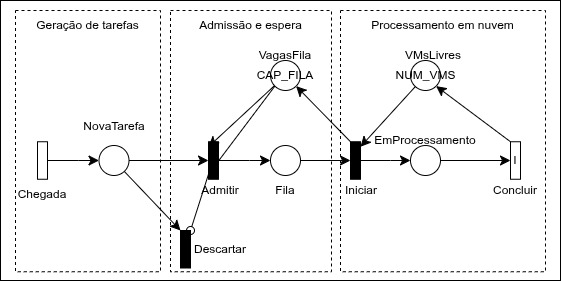
\includegraphics[width=\columnwidth]{modelo-spn.jpg}
    \caption{Modelo SPN do sistema de processamento de
    tarefas em nuvem. As marcações \texttt{CAP\_FILA}
    e \texttt{NUM\_VMS} representam as vagas disponíveis
    na fila e as VMs livres.}
    \label{fig:modelo-spn}
\end{figure}


Na área de geração de tarefas, a transição temporizada
\texttt{Chegada} representa o recebimento de requisições
enviadas pelos dispositivos clientes. Cada disparo produz
uma marca no lugar \texttt{NovaTarefa}, indicando uma tarefa
que aguarda a decisão de entrada no sistema. Consideram-se
intervalos entre chegadas exponenciais, com média
$1/\lambda$, sendo $\lambda$ a taxa de chegada definida
pelo parâmetro \texttt{TAXA\_CHEGADA}, em tarefas por segundo.

Na área de admissão e espera, o lugar \texttt{VagasFila}
representa a disponibilidade de posições na fila. Sua
marcação inicial é definida por \texttt{CAP\_FILA}, que
corresponde à capacidade máxima de espera. O lugar
\texttt{Fila} armazena as marcas das tarefas admitidas
que aguardam processamento. A transição imediata
\texttt{Admitir} consome uma marca de \texttt{NovaTarefa}
e uma de \texttt{VagasFila}, produzindo uma marca em
\texttt{Fila}. Dessa forma, a entrada de uma tarefa
ocupa uma posição de espera.

Quando todas as posições da fila estão ocupadas, o lugar
\texttt{VagasFila} fica sem marcas. Nessa condição, a
transição imediata \texttt{Descartar} remove a tarefa
de \texttt{NovaTarefa}. O arco inibidor entre
\texttt{VagasFila} e \texttt{Descartar}, com multiplicidade
unitária, estabelece que o descarte somente pode ocorrer
quando não existe uma posição disponível. Esse arco é
representado pelo círculo aberto em sua extremidade
na Figura~\ref{fig:modelo-spn}.

Na área de processamento em nuvem, o lugar
\texttt{VMsLivres} representa as máquinas virtuais
disponíveis, com marcação inicial definida por
\texttt{NUM\_VMS}. Uma tarefa em \texttt{Fila} inicia
o atendimento quando existe uma VM livre. A transição
imediata \texttt{Iniciar} consome uma marca de cada
um desses lugares e produz uma marca em
\texttt{EmProcessamento}. Ao mesmo tempo, devolve uma
marca a \texttt{VagasFila}, liberando a posição que
a tarefa ocupava na fila.

A conclusão do atendimento é representada pela transição
temporizada \texttt{Concluir}, que consome uma marca de
\texttt{EmProcessamento} e devolve uma marca a
\texttt{VMsLivres}. A tarefa deixa o sistema e a VM
fica disponível para um novo atendimento. Consideram-se
tempos de serviço exponenciais e independentes, com média
$S$, definida pelo parâmetro \texttt{TEMPO\_SERVICO}.
A política \textit{Infinite Server}, identificada pela
letra I, permite o processamento paralelo. A quantidade
de tarefas atendidas simultaneamente é limitada pelo
número de VMs representadas na rede.

Inicialmente, os lugares \texttt{NovaTarefa},
\texttt{Fila} e \texttt{EmProcessamento} estão vazios,
enquanto todas as vagas e VMs estão disponíveis.
Sejam $B$ a capacidade da fila e $n$ a quantidade de VMs.
Durante a execução, a soma das marcas de \texttt{Fila}
e \texttt{VagasFila} permanece igual a $B$. De forma
semelhante, a soma das marcas de \texttt{VMsLivres} e
\texttt{EmProcessamento} permanece igual a $n$.
Todos os arcos possuem multiplicidade unitária.

A Tabela~\ref{tab:metricas} apresenta as expressões das
cinco métricas utilizadas na avaliação. Nas expressões,
$L_q=E\{\#\texttt{Fila}\}$ representa a quantidade média
de tarefas em espera, e
$L_s=E\{\#\texttt{EmProcessamento}\}$ representa a
quantidade média de tarefas em atendimento.
O símbolo $\#$ indica a quantidade de marcas em um lugar,
$E\{\cdot\}$ indica seu valor médio estacionário e
$P\{\cdot\}$ indica a probabilidade da condição especificada.
Define-se ainda $p_f=P\{\#\texttt{VagasFila}=0\}$,
a probabilidade de a fila estar cheia.

\begin{table}[!t]
    \caption{Expressões das métricas utilizadas no modelo SPN.}
    \label{tab:metricas}
    \centering
    \footnotesize
    \renewcommand{\arraystretch}{1.4}
    \begin{tabularx}{\columnwidth}{@{}l c X@{}}
        \hline
        \textbf{Métrica} & \textbf{Expressão}
        & \textbf{Descrição e unidade} \\
        \hline
        $TP$ & $L_s/S$
        & Vazão de tarefas concluídas (tarefas/s) \\

        $MRT$ & $(L_q+L_s)/TP$
        & Tempo médio de resposta (s) \\

        $MQT$ & $L_q/TP$
        & Tempo médio de espera na fila (s) \\

        $U$ & $(L_s/n)\times 100$
        & Utilização média das VMs (\%) \\

        $DP$ & $p_f\times 100$
        & Probabilidade de descarte (\%) \\
        \hline
    \end{tabularx}
\end{table}

As expressões de tempo médio de resposta e de espera
aplicam a Lei de Little~\cite{little1961proof} às tarefas admitidas, utilizando
a vazão de conclusão como denominador. A probabilidade
de descarte é calculada pela fração do tempo em que
a fila está cheia. Sob a hipótese de chegadas de
Poisson independentes do estado do sistema, essa
fração corresponde à probabilidade de uma tarefa
recebida encontrar todas as posições de espera ocupadas~\cite{wolff1982poisson}.


\section{Simulações e resultados}
\label{sec:resultados}

Esta seção apresenta o planejamento experimental e os
resultados obtidos pela avaliação do modelo no Jupiter
Analytics. Os experimentos investigam os efeitos da demanda,
da quantidade de VMs e da capacidade da fila sobre o
desempenho. A análise considera as cinco métricas definidas
na Seção~\ref{sec:modelagem}.

\subsection{Configuração dos experimentos}

O cenário de referência utiliza três VMs, uma fila com
vinte posições, taxa média de chegada de vinte tarefas
por segundo e tempo médio de serviço de 0,1~s por tarefa.
O tempo de processamento e a capacidade de referência
da fila foram adaptados dos valores utilizados por
Macedo et al.~\cite{macedo2022vanets}. A interpretação
desses valores em um sistema de VMs constitui uma
hipótese do presente estudo.

Com tempo médio de serviço de 0,1~s, cada VM possui
capacidade nominal de dez tarefas por segundo. Dessa
forma, as três VMs do cenário de referência oferecem
capacidade nominal agregada de trinta tarefas por segundo.
A demanda de referência corresponde a aproximadamente
66,7\% dessa capacidade. Os níveis de chegada foram
selecionados para avaliar o sistema abaixo, próximo e
acima do limite nominal de processamento.
As configurações de duas, três e quatro VMs permitem
comparar a capacidade nominal igual e superior à demanda
de referência. As filas de dez, vinte e trinta vagas
avaliam a redução e a ampliação da capacidade de espera
em relação ao valor de referência.

A Tabela~\ref{tab:experimentos} apresenta os quatro
conjuntos de experimentos. Em cada conjunto, os
parâmetros que não são avaliados permanecem nos valores
de referência. No E4, demanda e recursos são aumentados
proporcionalmente, mantendo a carga oferecida igual
à capacidade nominal de processamento.

\begin{table}[!t]
    \caption{Planejamento experimental e cenário de referência.}
    \label{tab:experimentos}
    \centering
    \footnotesize
    \renewcommand{\arraystretch}{1.2}
    \begin{tabular}{c p{0.67\columnwidth}}
        \hline
        \textbf{Experimento} & \textbf{Configuração} \\
        \hline
        Referência &
        $\lambda=20$ tarefas/s; $n=3$; $B=20$;
        $S=0,1$~s \\

        E1 &
        $\lambda \in \{10,20,30,40,50\}$ tarefas/s \\

        E2 &
        $n \in \{2,3,4\}$ VMs \\

        E3 &
        $B \in \{10,20,30\}$ vagas \\

        E4 &
        $(\lambda,n)\in\{(20,2),(30,3),(40,4)\}$ \\
        \hline
    \end{tabular}
\end{table}

As avaliações foram realizadas por simulação estacionária,
com horizonte de 10.000~s e período de aquecimento de
1.000~s. Foram configurados nível de confiança de 95\%,
erro relativo máximo de 5\% e limite de vinte milhões
de eventos. Na execução individual utilizada para completar
o ponto de quarenta tarefas por segundo com seis VMs,
o limite de tempo computacional foi ampliado para
300~s após a ocorrência de interrupção por tempo excedido.

Os resultados de E1 a E4 foram consolidados a partir
das tabelas apresentadas pelo Jupiter. Na análise
comparativa, foram utilizados arquivos CSV exportados
pela ferramenta. O ponto de quarenta tarefas por segundo
com seis VMs foi obtido em uma execução individual e
transcrito com a precisão de quatro casas decimais
exibida pela interface.

Os gráficos apresentam estimativas pontuais. Os arquivos
utilizados na elaboração das figuras não contêm os
limites dos intervalos de confiança, o que restringe a
interpretação de diferenças pequenas entre configurações.

\subsection{Efeito da demanda}

No E1, a taxa de chegada varia de dez a cinquenta tarefas
por segundo, mantendo três VMs e vinte vagas na fila.
O tempo médio de resposta aumenta de 0,1045~s para
0,7167~s nesse intervalo. Com dez tarefas por segundo,
a espera média é de 0,0045~s, indicando que a maior
parte do tempo de resposta corresponde ao processamento.

Quando a demanda atinge trinta tarefas por segundo,
a utilização chega a 95,6658\%, o tempo médio de resposta
atinge 0,4200~s e o descarte alcança 4,3702\%.
Com cinquenta tarefas por segundo, a utilização fica
próxima de 100\%, enquanto a vazão permanece em
aproximadamente trinta tarefas por segundo e o descarte
atinge 40,0052\%. Esses resultados identificam as VMs
como o principal limite de processamento nessa configuração.

O aumento da demanda após a saturação provoca maior
ocupação da fila e rejeição de tarefas. A capacidade
finita de espera também limita o crescimento do tempo
médio de resposta das tarefas admitidas. Portanto,
a interpretação dessa métrica deve considerar
simultaneamente a probabilidade de descarte.

\subsection{Efeito da quantidade de VMs}

No E2, são comparadas duas, três e quatro VMs, mantendo
a demanda em vinte tarefas por segundo. Com duas VMs,
o tempo médio de resposta é de 0,5896~s e a utilização
atinge 95,5703\%. O descarte nessa configuração
corresponde a 4,4976\%.

Ao aumentar a capacidade para três VMs, o tempo médio
de resposta diminui para 0,1445~s, uma redução de
aproximadamente 75,5\%. A espera média passa de
0,4896~s para 0,0445~s, evidenciando que a melhoria
decorre da redução da contenção pelos recursos.
O descarte diminui para 0,0042\%.

Com quatro VMs, o tempo médio de resposta chega a
0,1087~s e a utilização média é de 50,0033\%.
A redução adicional do tempo de resposta é de
aproximadamente 24,8\% em relação à configuração
com três VMs. Nesse cenário, o tempo de resposta
já se aproxima do tempo médio de serviço de 0,1~s.

\subsection{Efeito da capacidade da fila}

A Figura~\ref{fig:e3} apresenta o E3, no qual a capacidade
da fila assume dez, vinte e trinta vagas. A demanda
permanece em vinte tarefas por segundo e são utilizadas
três VMs.

\begin{figure}[!t]
    \centering
    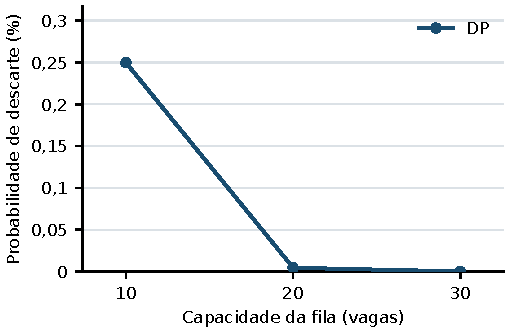
\includegraphics[width=\columnwidth]{e3-fila.pdf}
    \caption{Probabilidade de descarte em função da
    capacidade da fila, com três VMs, chegada de vinte
    tarefas por segundo e serviço médio de 0,1~s.}
    \label{fig:e3}
\end{figure}

Com dez vagas, a probabilidade de descarte é de 0,2498\%.
Ao ampliar a fila para vinte vagas, esse valor diminui
para 0,0045\%. Com trinta vagas, a estimativa exibida
é de 0,0001\%. O tempo médio de resposta passa de
0,1412~s para 0,1445~s entre os extremos avaliados.

O crescimento da fila permite admitir tarefas que
seriam rejeitadas por falta de espaço. Essas tarefas
podem permanecer em espera, o que explica o pequeno
aumento observado no tempo de resposta. A ampliação
da fila atua sobre a capacidade de acomodação,
enquanto a capacidade nominal de processamento
permanece determinada pelas três VMs.

\subsection{Demanda e recursos combinados}

No E4, são avaliados os pares de demanda e quantidade
de VMs apresentados na Tabela~\ref{tab:resultados-e4}.
A fila permanece com vinte vagas e o tempo médio
de serviço é mantido em 0,1~s.

\begin{table}[!t]
    \caption{Parâmetros e resultados dos cenários combinados.}
    \label{tab:resultados-e4}
    \centering
    \footnotesize
    \renewcommand{\arraystretch}{1.2}
    \begin{tabular}{l r r r}
        \hline
        \textbf{Parâmetro ou métrica}
        & \textbf{E4.1} & \textbf{E4.2} & \textbf{E4.3} \\
        \hline
        Chegada (tarefas/s) & 20 & 30 & 40 \\
        Quantidade de VMs & 2 & 3 & 4 \\
        Vagas na fila & 20 & 20 & 20 \\
        Serviço médio (s) & 0,1 & 0,1 & 0,1 \\
        Vazão (tarefas/s) & 19,1129 & 28,6823 & 38,2899 \\
        Resposta (s) & 0,5896 & 0,4197 & 0,3367 \\
        Espera (s) & 0,4896 & 0,3197 & 0,2367 \\
        Utilização (\%) & 95,5643 & 95,6076 & 95,7247 \\
        Descarte (\%) & 4,4604 & 4,3633 & 4,3282 \\
        \hline
    \end{tabular}
\end{table}

A Figura~\ref{fig:e4} mostra a redução do tempo médio
de resposta entre os cenários combinados. Embora a
demanda aumente, a quantidade de recursos também cresce,
e o tempo médio de resposta diminui de 0,5896~s para
0,3367~s. A utilização permanece próxima de 95,6\%
nas três configurações, e as estimativas de descarte
ficam próximas de 4,4\%.

\begin{figure}[!t]
    \centering
    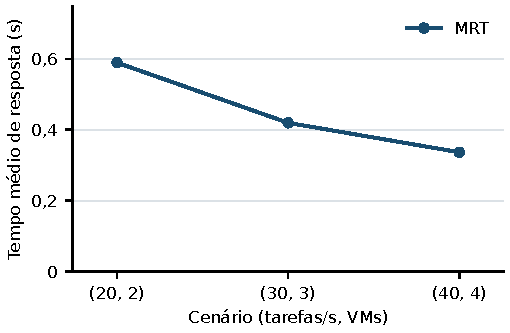
\includegraphics[width=\columnwidth]{e4-demanda-e-vms.pdf}
    \caption{Tempo médio de resposta nos cenários
    combinados. Cada par indica a taxa de chegada,
    em tarefas por segundo, e a quantidade de VMs.}
    \label{fig:e4}
\end{figure}

Os resultados mostram que ampliar proporcionalmente
demanda e recursos pode reduzir a espera em um sistema
com múltiplos atendimentos paralelos. A manutenção
de descarte nesses cenários também indica que operar
com carga oferecida igual à capacidade nominal deixa
o sistema sujeito à contenção provocada pela
variabilidade das chegadas e dos serviços.


\subsection{Comparação das configurações de capacidade}

Uma análise complementar avalia cinco configurações,
com duas a seis VMs, sob taxas de chegada de dez a
cinquenta tarefas por segundo. As Figuras~\ref{fig:comparativo-u} a~\ref{fig:comparativo-mqt}
apresentam os resultados, mantendo vinte vagas na fila
e tempo médio de serviço de 0,1~s.


A Figura~\ref{fig:comparativo-u} mostra o crescimento
da utilização com a demanda. Para uma mesma taxa
de chegada, configurações com maior quantidade de VMs
apresentam menor ocupação média. Com duas VMs,
a utilização se aproxima de 100\% a partir de trinta
tarefas por segundo. Com seis VMs e cinquenta tarefas
por segundo, a utilização é de aproximadamente 83,14\%,
indicando maior margem de processamento.

\begin{figure}[!ht]
    \centering
    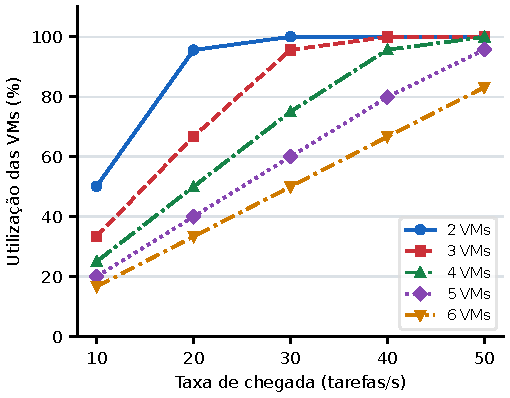
\includegraphics[width=\columnwidth]{comparativo-u.pdf}
    \caption{Utilização das VMs em função da taxa de chegada
    para duas a seis VMs, com fila de vinte vagas
    e serviço médio de 0,1~s.}
    \label{fig:comparativo-u}
\end{figure}


A Figura~\ref{fig:comparativo-mrt} apresenta o tempo
médio de resposta. Com quarenta tarefas por segundo,
três VMs apresentam resposta de 0,6679~s. Com quatro
VMs, esse valor diminui para 0,3361~s, e com seis
VMs chega a 0,1142~s. O crescimento da capacidade
permite atender uma parcela maior da demanda com
menor tempo de espera.

\begin{figure}[!ht]
    \centering
    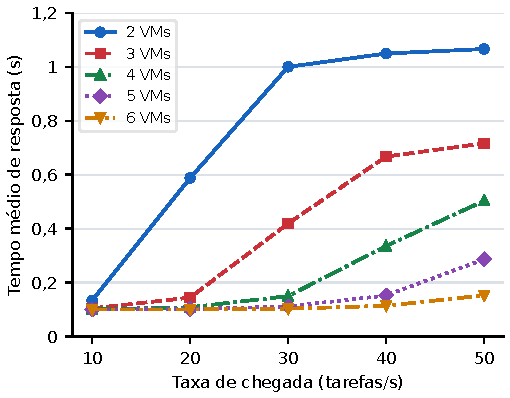
\includegraphics[width=\columnwidth]{comparativo-mrt.pdf}
    \caption{Tempo médio de resposta em função da taxa de chegada
    para duas a seis VMs, com fila de vinte vagas
    e serviço médio de 0,1~s.}
    \label{fig:comparativo-mrt}
\end{figure}


A Figura~\ref{fig:comparativo-dp} apresenta o efeito
da capacidade sobre o descarte. Para quarenta tarefas
por segundo, três VMs apresentam descarte de
24,9934\%. Com quatro VMs, esse valor diminui para
4,2987\%, enquanto seis VMs apresentam 0,0027\%.
O resultado evidencia que a capacidade adicional
reduz a frequência com que as chegadas encontram
a fila cheia.

\begin{figure}[!ht]
    \centering
    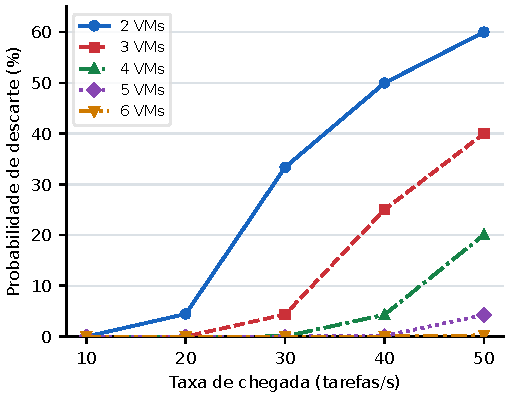
\includegraphics[width=\columnwidth]{comparativo-dp.pdf}
    \caption{Probabilidade de descarte em função da taxa de chegada
    para duas a seis VMs, com fila de vinte vagas
    e serviço médio de 0,1~s.}
    \label{fig:comparativo-dp}
\end{figure}


A Figura~\ref{fig:comparativo-mqt} mostra o tempo
médio de espera. Para quarenta tarefas por segundo,
a espera diminui de aproximadamente 0,5679~s com
três VMs para 0,0142~s com seis VMs. Como o tempo
médio de serviço permanece em 0,1~s, a redução
da espera explica a melhoria observada no tempo
de resposta.

\begin{figure}[!ht]
    \centering
    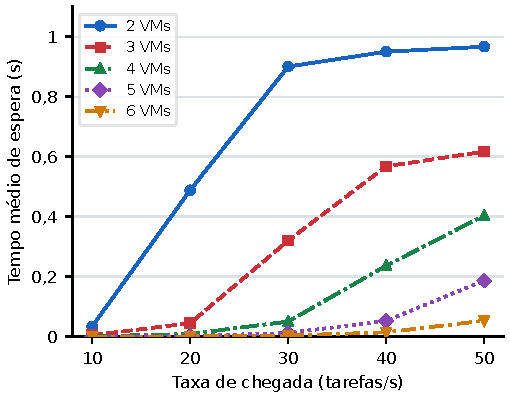
\includegraphics[width=\columnwidth]{comparativo-mqt.pdf}
    \caption{Tempo médio de espera em função da taxa de chegada
    para duas a seis VMs, com fila de vinte vagas
    e serviço médio de 0,1~s.}
    \label{fig:comparativo-mqt}
\end{figure}


Para a demanda de referência de vinte tarefas por
segundo, três VMs constituem uma alternativa de
equilíbrio entre quantidade de recursos e desempenho.
No E2, essa configuração mantém utilização de
66,6829\%, tempo médio de resposta de 0,1445~s
e descarte de 0,0042\%. Uma quarta VM reduz a espera,
mas também diminui a utilização média para
aproximadamente 50\%.

A recomendação depende da demanda esperada e dos
requisitos de resposta e rejeição. Entre as configurações
avaliadas, seis VMs oferecem maior margem de capacidade
para demandas elevadas. Já no cenário de referência,
três VMs apresentam desempenho próximo do tempo de
serviço com menor quantidade de recursos. Essa
interpretação utiliza o número de VMs como indicador
de recursos alocados, pois o estudo não estabelece
um modelo monetário de custos.

\section{Conclusão}
\label{sec:conclusao}

Este trabalho apresentou um modelo SPN para avaliar o
desempenho de um sistema de processamento de tarefas em
nuvem, composto por VMs idênticas e uma fila compartilhada
de capacidade limitada. O modelo foi implementado no
Jupiter Analytics e avaliado por simulação estacionária.
Os experimentos consideraram alterações na demanda,
na quantidade de VMs, na capacidade da fila e em
combinações de demanda e recursos.

Os resultados mostraram que o aumento da taxa de chegada
eleva a utilização, a espera e o descarte quando a demanda
se aproxima ou ultrapassa a capacidade de processamento.
Com três VMs e cinquenta tarefas por segundo, a vazão
permaneceu próxima de trinta tarefas por segundo,
enquanto o descarte atingiu aproximadamente 40\%.
Esse comportamento identificou os recursos de
processamento como o principal gargalo dessa configuração.

A ampliação da quantidade de VMs reduziu o tempo de
resposta e a probabilidade de descarte para uma mesma
demanda. No cenário de referência, com vinte tarefas
por segundo e vinte vagas na fila, três VMs apresentaram
tempo médio de resposta de 0,1445~s, utilização de
66,6829\% e descarte de 0,0042\%. Essa configuração
constitui uma alternativa de equilíbrio entre recursos
alocados e desempenho para a carga estudada. Uma quarta
VM reduziu a resposta para 0,1087~s, acompanhada de
utilização próxima de 50\%.

A ampliação da fila também reduziu o descarte, mas
produziu um pequeno aumento no tempo médio de resposta
das tarefas admitidas. Dessa forma, o dimensionamento
deve considerar conjuntamente a quantidade de VMs
e a capacidade de espera. Para demandas mais elevadas,
a comparação entre cinco configurações mostrou que
recursos adicionais ampliam a margem de atendimento
e reduzem a contenção.

As conclusões estão restritas às hipóteses de VMs
idênticas, chegadas de Poisson e tempos de serviço
exponenciais, com parâmetros adaptados da literatura.
Os resultados apresentados são estimativas pontuais,
e o estudo utiliza a quantidade de VMs como indicador
de recursos alocados. Como trabalhos futuros,
propõem-se a calibração do modelo com medições de
uma aplicação real, a avaliação de cargas variáveis
ao longo do tempo e a inclusão de custos para apoiar
a escolha das configurações.


O modelo, as configurações dos experimentos e os resultados
estão disponíveis no \href{https://github.com/RaisSousaa/Trabalho07-SD}{repositório do projeto no GitHub}.
A apresentação em vídeo pode ser acessada pelo
\href{https://drive.google.com/file/d/1r0zUEZ-HTNkOxSzZm_K4DD1HS4JBRgOu/view?usp=sharing}{Google Drive}.

\bibliographystyle{IEEEtran}
\bibliography{referencias}
\end{document}
